\chapter{Week}
In this week I started working on the second presentation 'Introduction to \ac{ML} on \acp{FPGA}'. This time the focus should be on the hardware needed to handle typical \ac{ML} workloads, namely inference and training along all major fields of applications where \ac{ANN} are used. The main areas are: image classification, object detection, semantic segmentation, optical character recognition and speech recognition. The presentation structure is as follows:
\begin{itemize}
	\item \textbf{\ac{ANN} workload:} Using a state-of-the-art neural network (resnet50) the number of operations per image were illustrated to show the vast amount of compute and memory needed for a single image. This was done for inference and training respectively with the purpose of driving home the challenges involved in \ac{ML} applications. Moreover, the majority of operations are costly \ac{MAC} operations which take several clock cycles to complete.
	\item \textbf{Hardware for training:} The industry right now in terms of \ac{ANN} training is dominated by NVIDIA and so the clear answer here was \ac{GPU}. There are a number of start-ups developing alternative solutions to get into the \ac{ANN} training market. The main advantage these start-ups have is that they can design from scratch and use an architecture tailored to the specific requirements of \ac{ANN} training. The sheer number of floating point 32 operations and the requirements for memory are strictly not suited for \acp{FPGA}.
	\item \textbf{Hardware for inference:} The picture is different for inference. Here, a lot of research has been done in using quantization and pruning of \ac{ANN} models without impeding the performance of these networks. The reason for this is, that neural networks are inherently over-parametrized and this is necessary for the training algorithms to work. Once a trained network is obtained however, the network can be compressed severely (up to 90 \%) without network degradation. A qualitative comparison of the available platforms was made to show the strengths and weaknesses of each platform. The flexibility of \acp{FPGA} make them a suitable platform for \ac{ANN} inference.
	\item \textbf{\ac{FPGA} architecture:} Figure~\ref{fig:fpga_arch} shows the two possible high-level architectures that are typically used in neural network implementations. On the left you have the streaming architecture where basically the structure of the neural network is mirrored by the hardware implementation. The main benefit is the efficiency and customizability as the hardware can be tailored specifically to each network. The other approach is shown on the right. This is a more general approach in that it has a single computation engine which breaks down the operations needed for neural network inference. These operations are controlled by a host and executed on demand. The main benefit here is the flexibility. As the types of layers in a neural network are fixed, efficient implementation of these different types of layers enables the deployment of arbitrary neural networks. The downside is that the implementation is limited by the architecture in terms of tailoring the hardware implementation to the neural network.
	\begin{figure}[!htb]
	\centering
		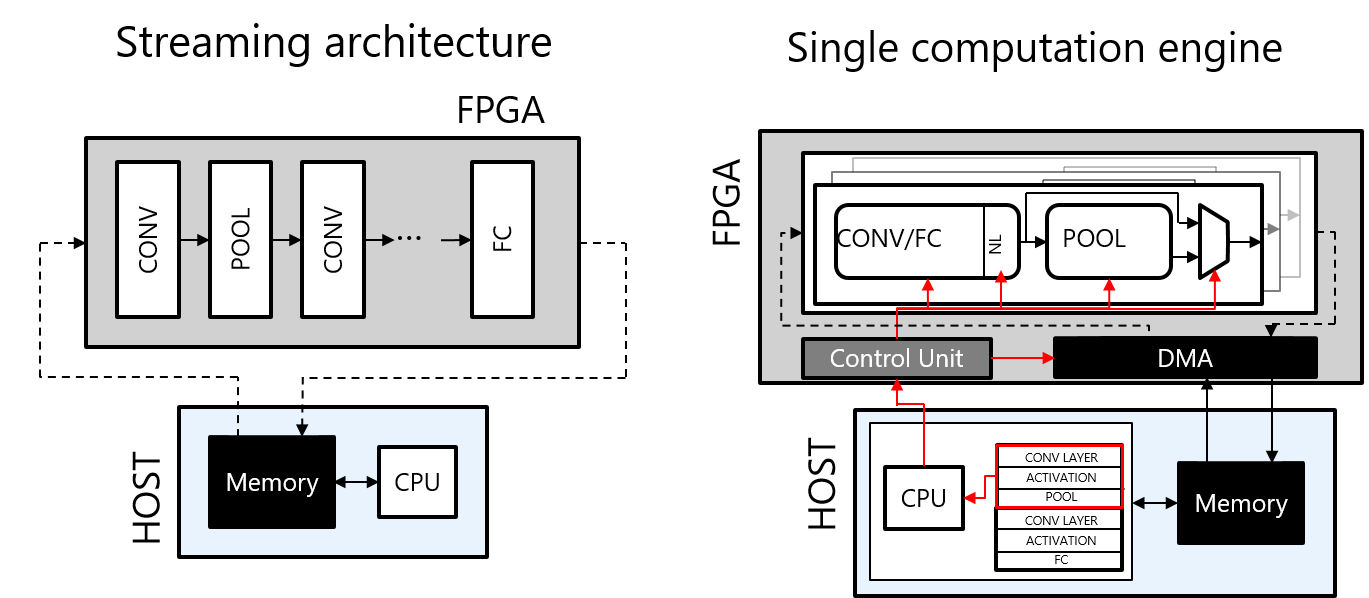
\includegraphics[width=\textwidth]{bilder/FPGA_arch.png}
		\caption{\acs{FPGA} architecture overview}
		\label{fig:fpga_arch}
\end{figure}
	\item \textbf{\ac{DNNDK} work flow:} Lastly, the \ac{DNNDK} work flow is introduced with a focus on adjusting the \ac{DPU} \ac{IP} core to custom boards. Some demonstrations implemented on the ZCU 104 evaluation board were used to finish the presentation and show the employees, what is possible with the tools available.
\end{itemize}
In this week on Thursday there was a Xilinx \ac{ML} seminar in Munich, where I went to with my supervisor to get more information about Xilinx \ac{AI} solutions. This was a whole day event with several segments, showing off the capabilities and the work flow of Xilinx cloud and edge \ac{AI} tools. This was also a great opportunity for networking and speaking in person to top Xilinx \ac{FAE} engineers.